\chapter{Примеры использования и перспективы}\label{chapter-usage}

\section{Получение числа π методом Гальперина}\label{pipool}

Реализованную симуляцию можно использовать для вычисления числа \(\pi\)
методом Г.~Гальперина~\cite{poolpi}.
Этот метод заключается в том, что в системе из стенки слева,
тела массой \(1\) и телом массой \(100^{n - 1}\) эти тела соударяются и число этих столкновений
будет равно первым \(n\) цифрам числа~\(\pi\)~\cite{habrpi}.
При этом, в системе нет трения, т.е. сталкиваться тела закончат, когда оба улетят вправо, причём у тела с меньшей массой скорость будет меньше.
Разработанный движок хоть и рассчитан на движение с трением, но может и без него, если коэффициент трения сделать равным нулю.

Например, рассчитать первые 4 цифры можно следующим образом.
Очистить модель, поставить воспроизведение на паузу и отмотать время в ноль~(рисунок~\ref{pistep1fig}).

\begin{figure}[H]
    \centering
    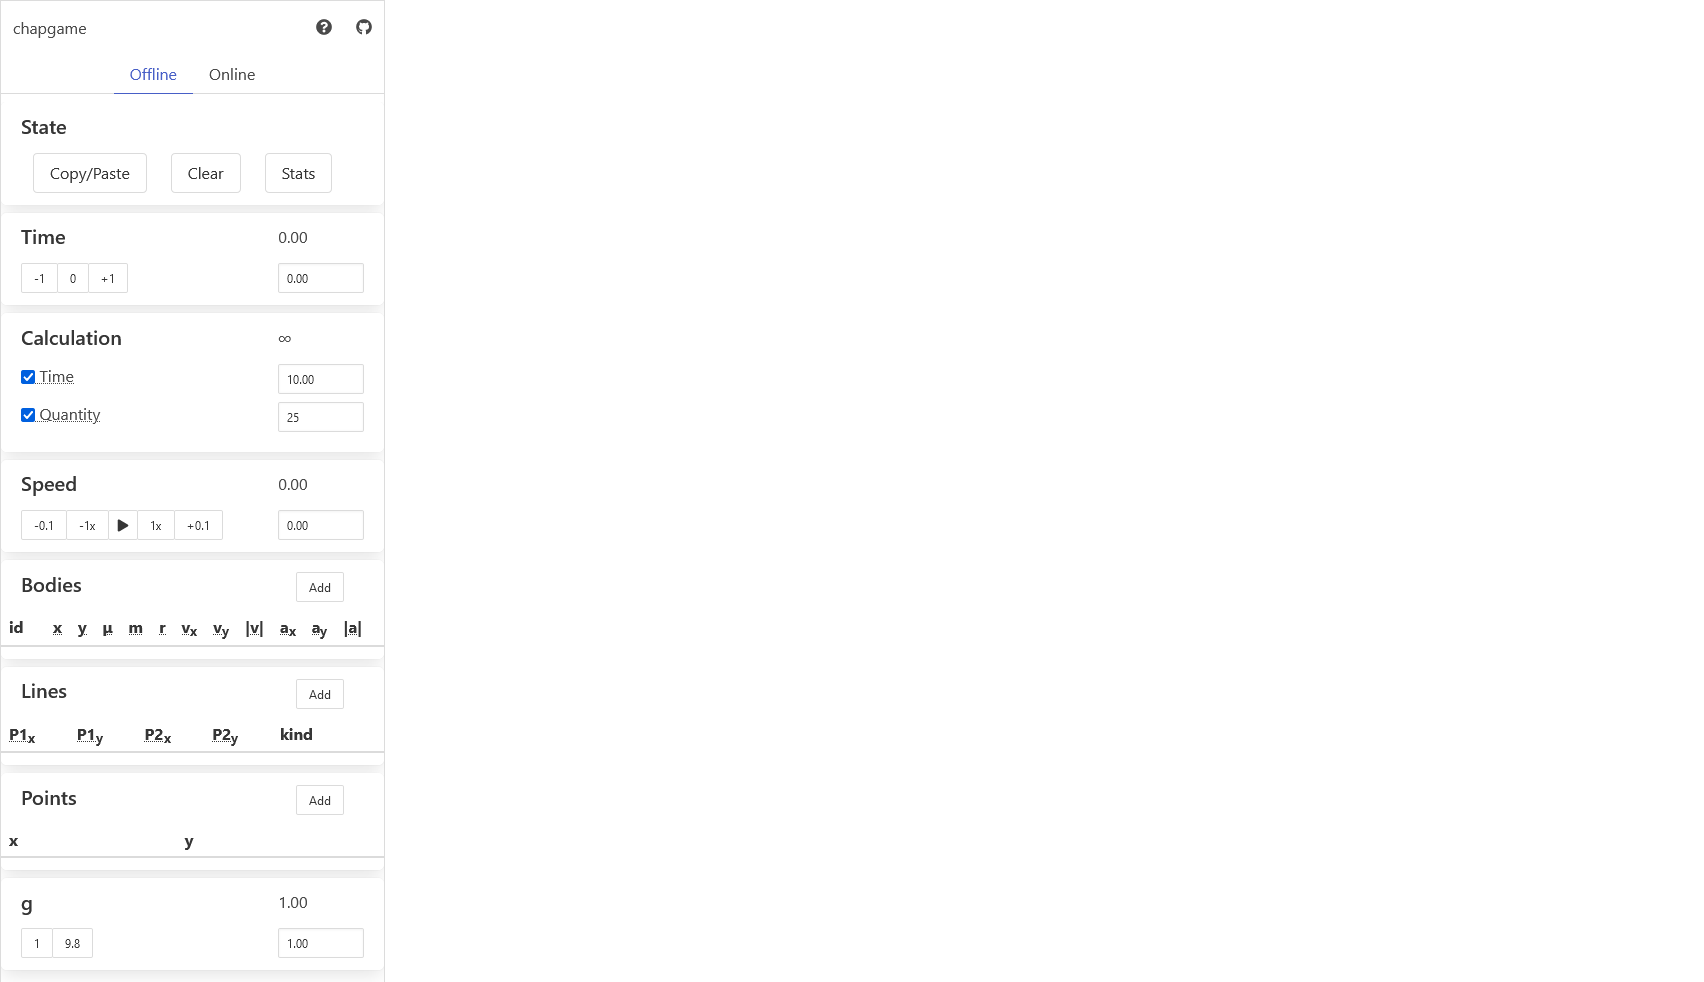
\includegraphics[width=16cm]{pistep1}
    \caption{Шаг 1\label{pistep1fig}}
\end{figure}

Добавить вертикальную линию, которая будет располагаться слева от тел~(рисунок~\ref{pistep2fig}).

\begin{figure}[H]
    \centering
    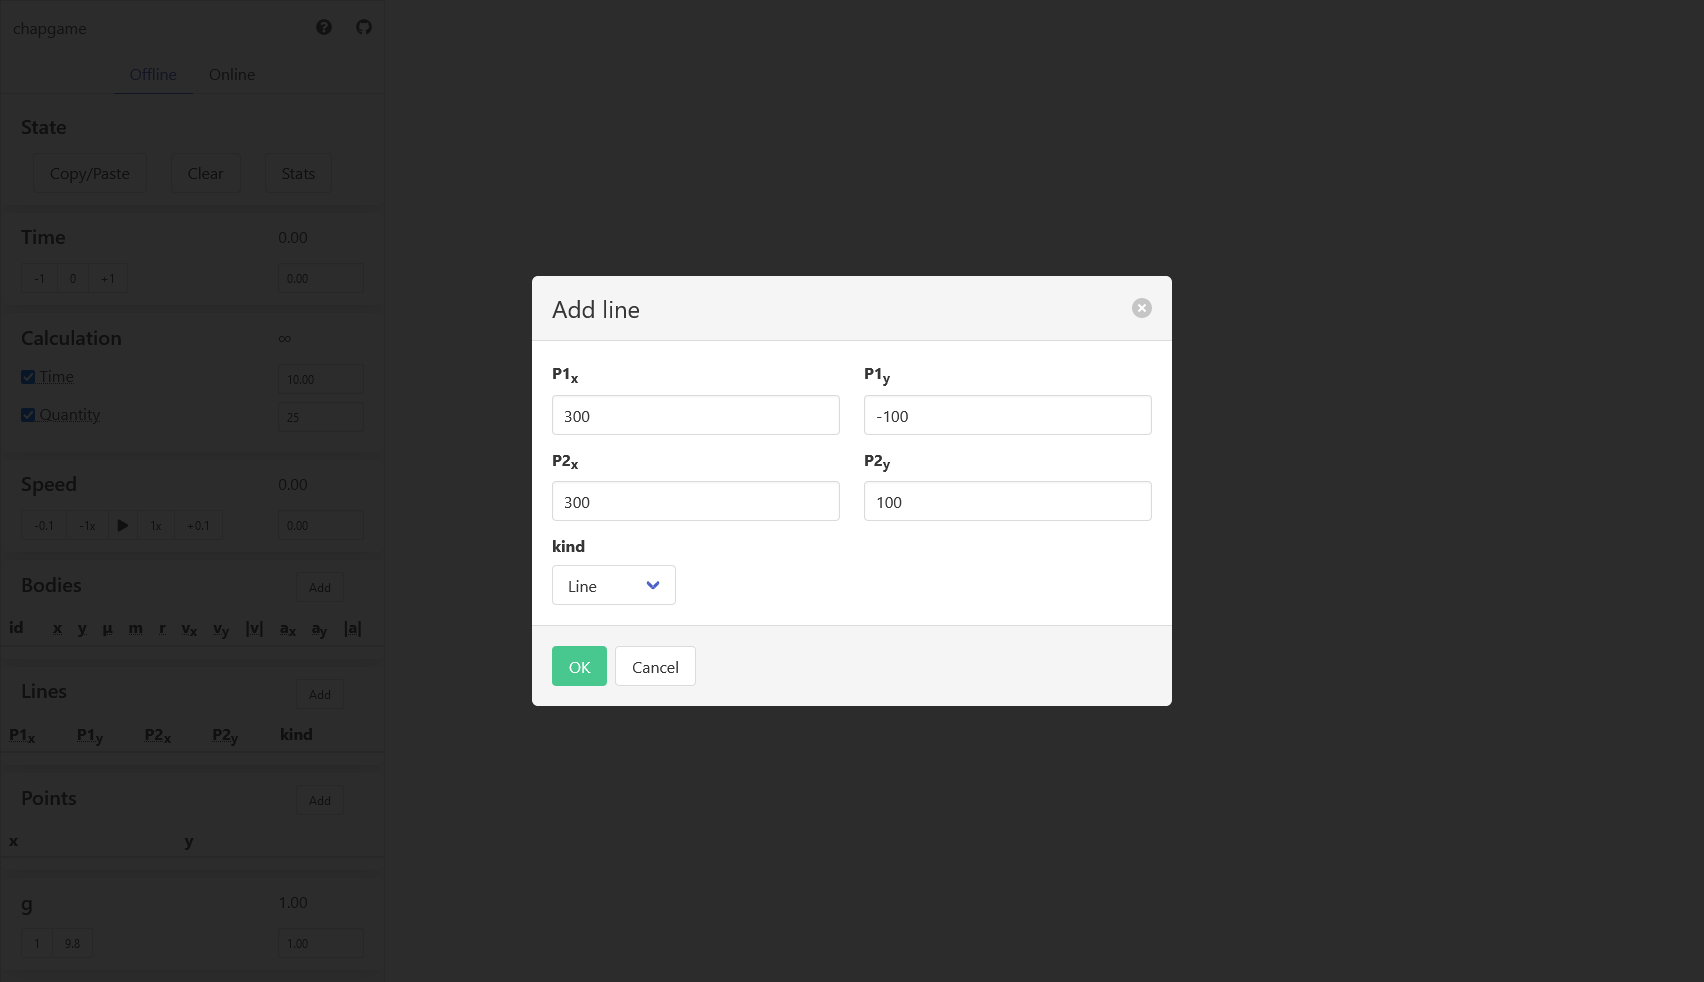
\includegraphics[width=16cm]{pistep2}
    \caption{Шаг 2\label{pistep2fig}}
\end{figure}

Добавить тело с меньшей массой~(рисунок~\ref{pistep3fig}).
Так как оно должно быть правее добавленной линии, координата по оси \(X\)
добавляемого тела должна быть больше.

\begin{figure}[H]
    \centering
    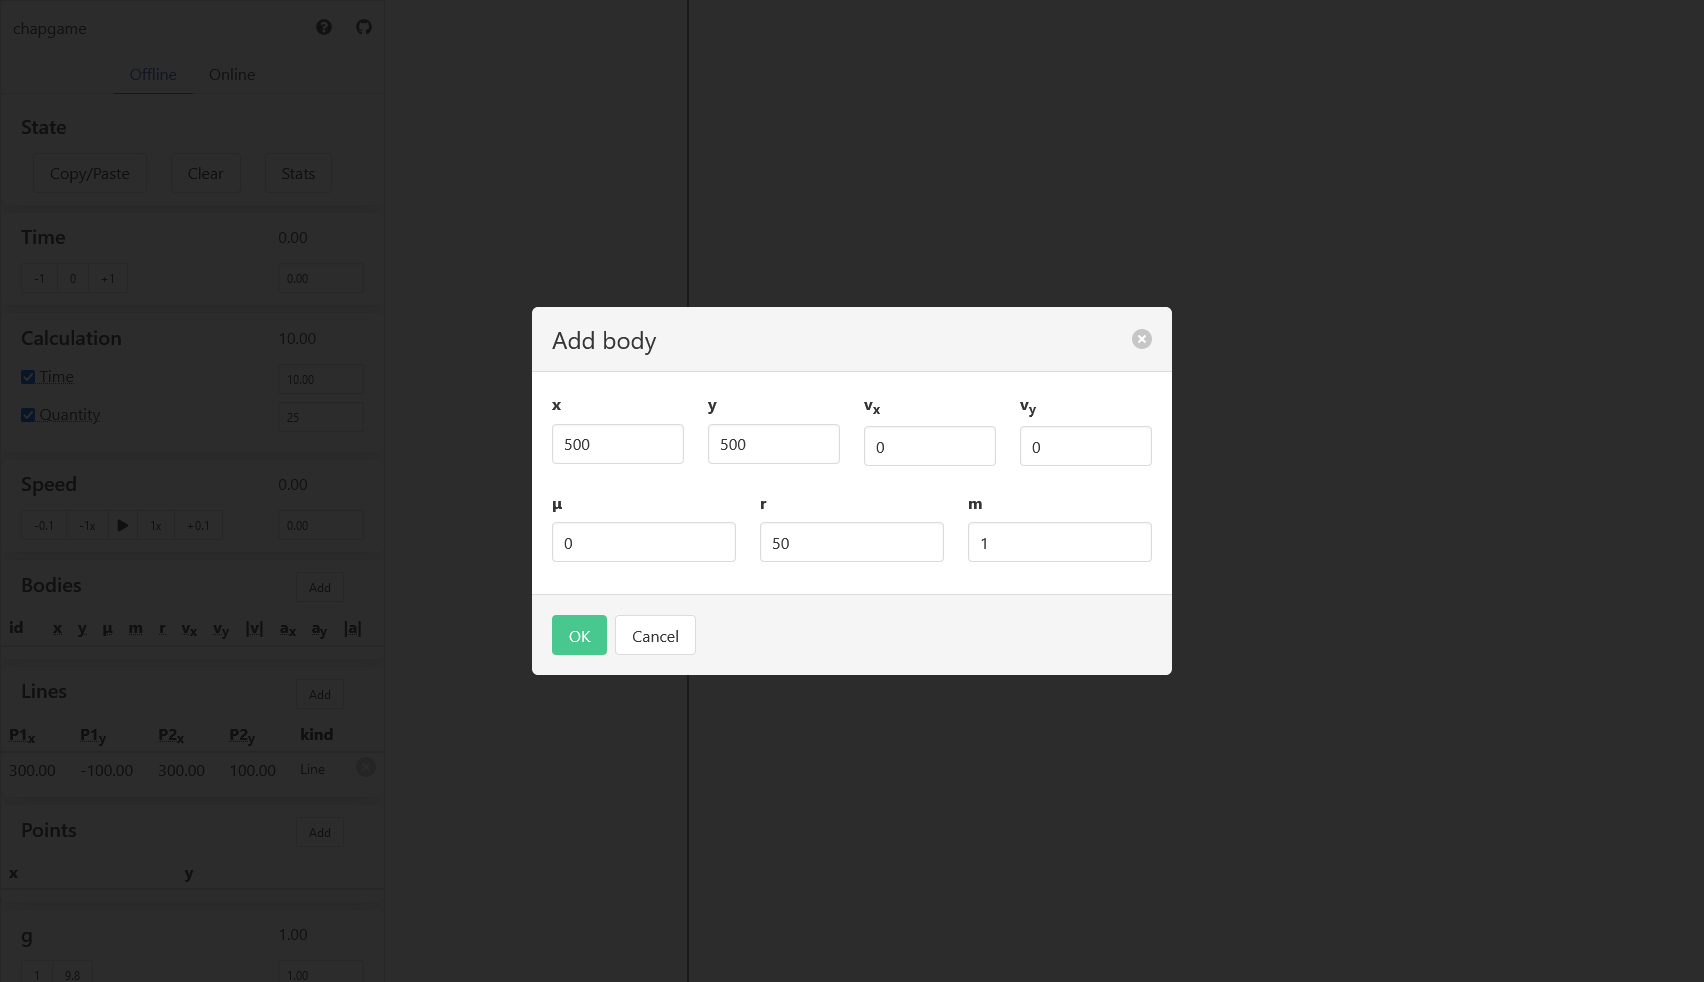
\includegraphics[width=16cm]{pistep3}
    \caption{Шаг 3\label{pistep3fig}}
\end{figure}

Добавить тело с большей массой, его координата по оси \(X\) должна быть ещё больше;
радиус можно оставить таким же, а масса должна быть в \(100^3\) раз больше так как требуется вычислить 4 цифры;
скорость этого тела должна быть направлена влево (рисунок~\ref{pistep4fig}).

\begin{figure}[H]
    \centering
    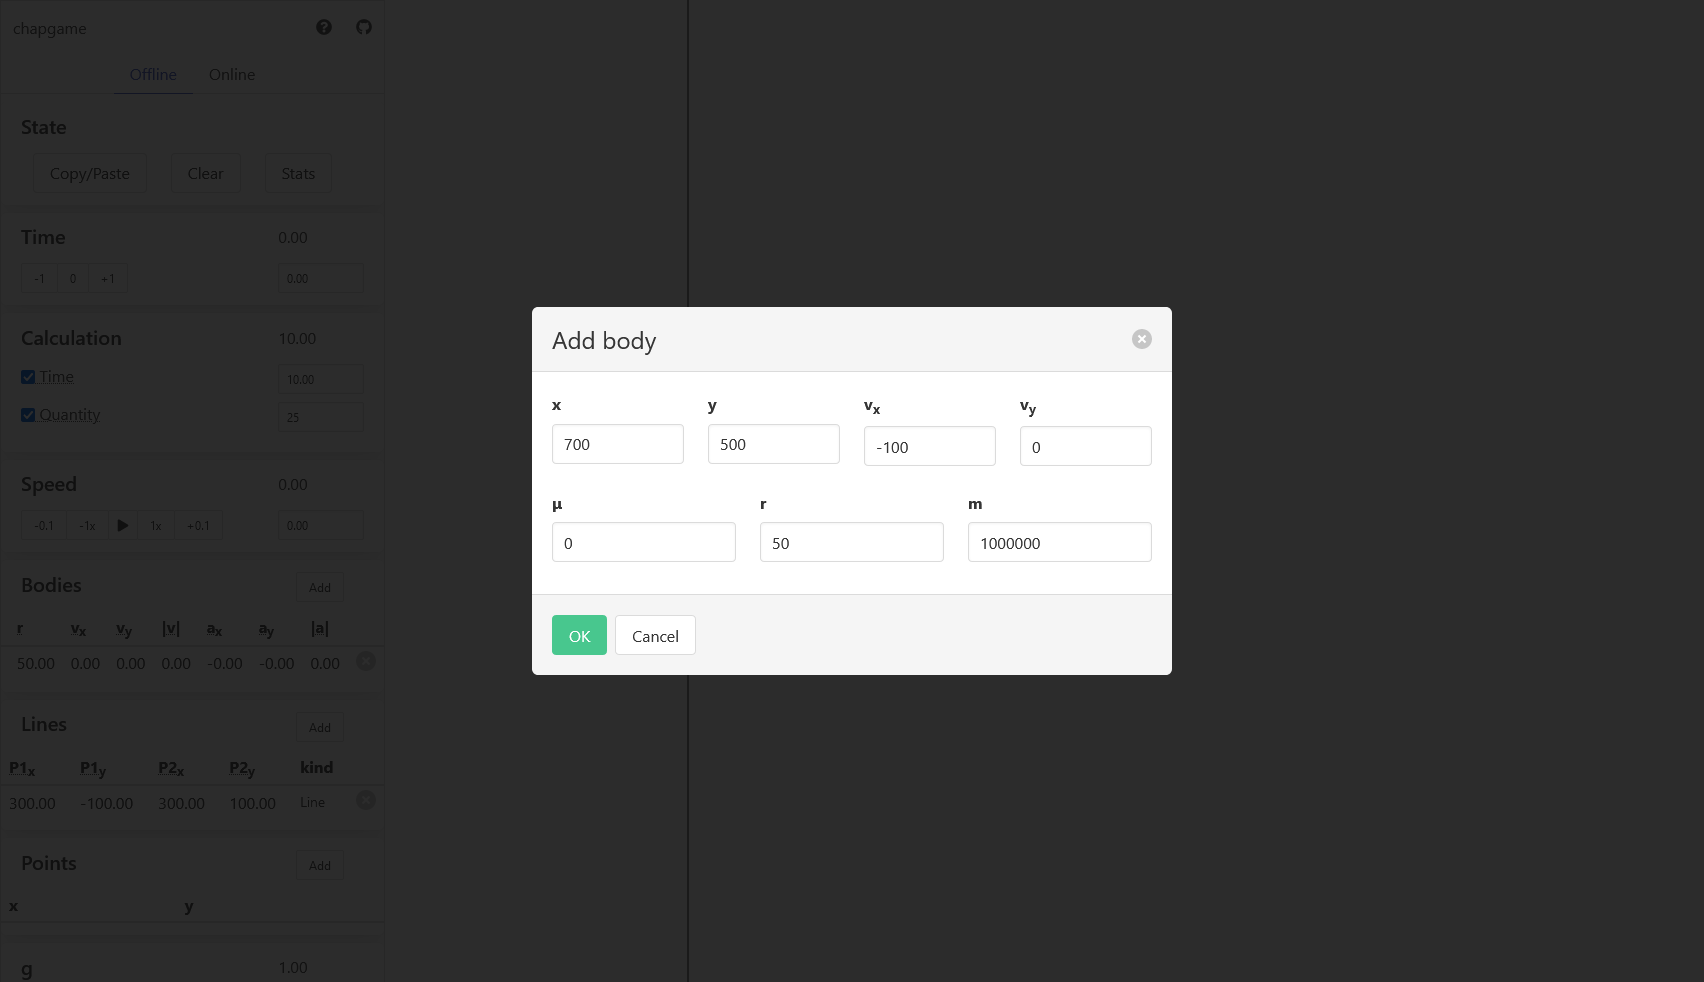
\includegraphics[width=16cm]{pistep4}
    \caption{Шаг 4\label{pistep4fig}}
\end{figure}

Убрать галочки, отвечающие за параметры расчёта, чтобы модель рассчиталась до конца~(рисунок~\ref{pistep5fig}).

\begin{figure}[H]
    \centering
    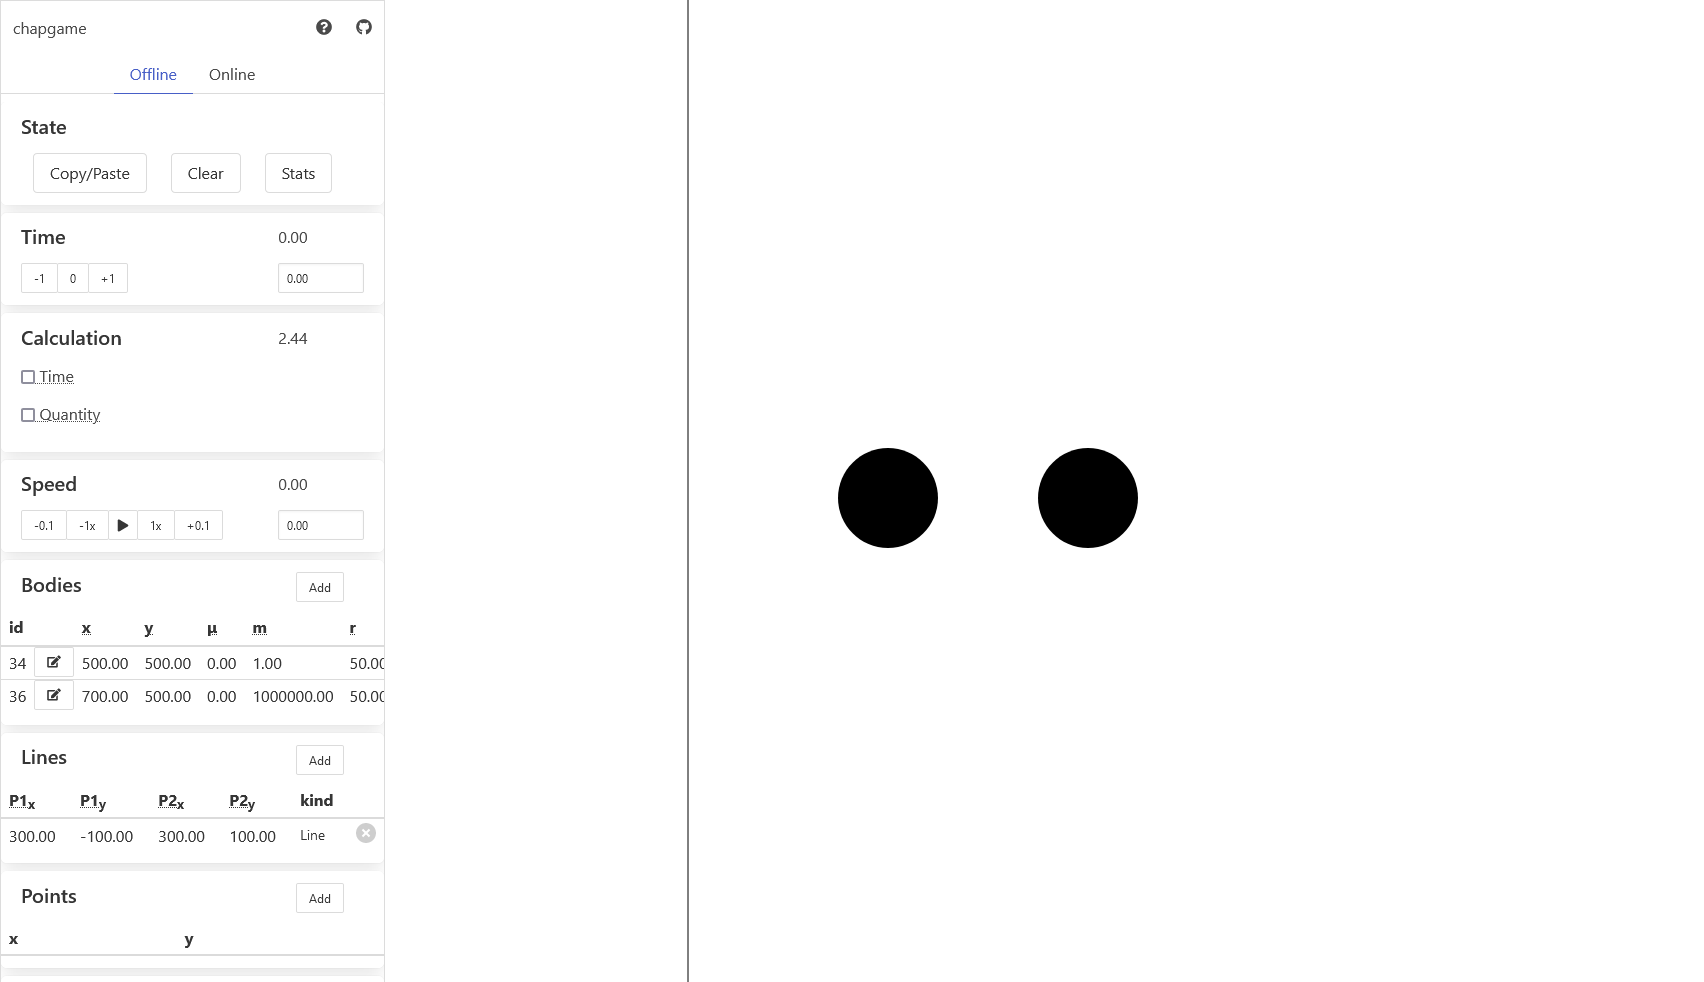
\includegraphics[width=16cm]{pistep5}
    \caption{Шаг 5\label{pistep5fig}}
\end{figure}

Снять воспроизведение с паузы и дождаться когда произойдёт расчёт. Можно наблюдать за столкновениями,
или сразу открыть статистику и в счётчике столкновений будет искомое число: \(3141\), что является
первыми 4 цифрами числа \(\pi \approx 3.14159265359\) (рисунок~\ref{pistep6fig}).

\begin{figure}[H]
    \centering
    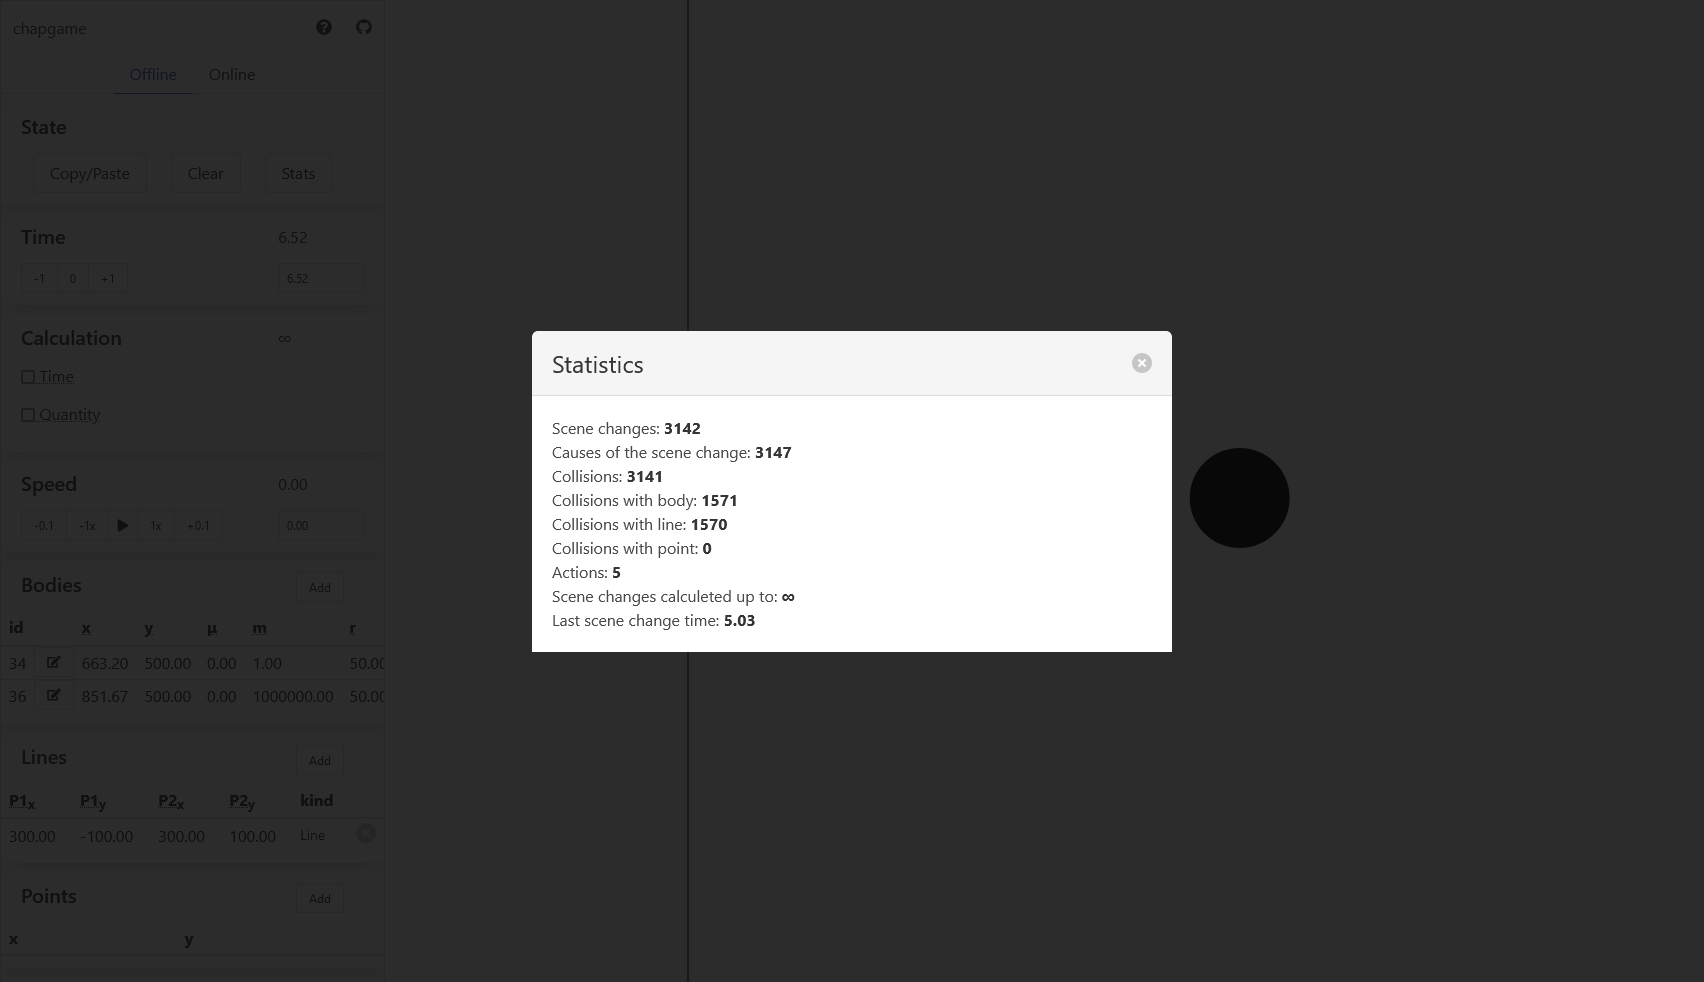
\includegraphics[width=16cm]{pistep6}
    \caption{Шаг 6\label{pistep6fig}}
\end{figure}

\section{Визуализация броуновского движения}

Броуновское движение~-- хаотическое перемещение очень малых частиц вещества под действием ударов молекул~\cite{browniankrugosvet}.
Столкновения молекул можно визуализировать реализованным движком.
Однако, асимптотическая сложность реализованного алгоритма равна~(\ref{onmk}), так как требуется перебирать все пары тело-тело, тело-линия, тело-точка.

\begin{equation}\label{onmk}
    O(n(n + m + k))
\end{equation}

\begin{Underequation}
    \(n\)~-- количество тел;

    \(m\)~-- количество линий;

    \(k\)~-- количество точек.
\end{Underequation}

Поэтому, когда в модели слишком много объектов, вычисления идут намного медленнее, а для визуализации броуновского движения желательно использовать много тел (частиц).
Это можно можно будет смягчить, оптимизировав алгоритм. Возможные оптимизации рассмотрены далее в пункте~\ref{optimization}.
Но всё равно на рисунке~\ref{brownianfig} представлена раскадровка с шагом в \(0.1\) секунду визуализации условного броуновского движения с 15 частицами.

\begin{figure}[H]
    \centering
    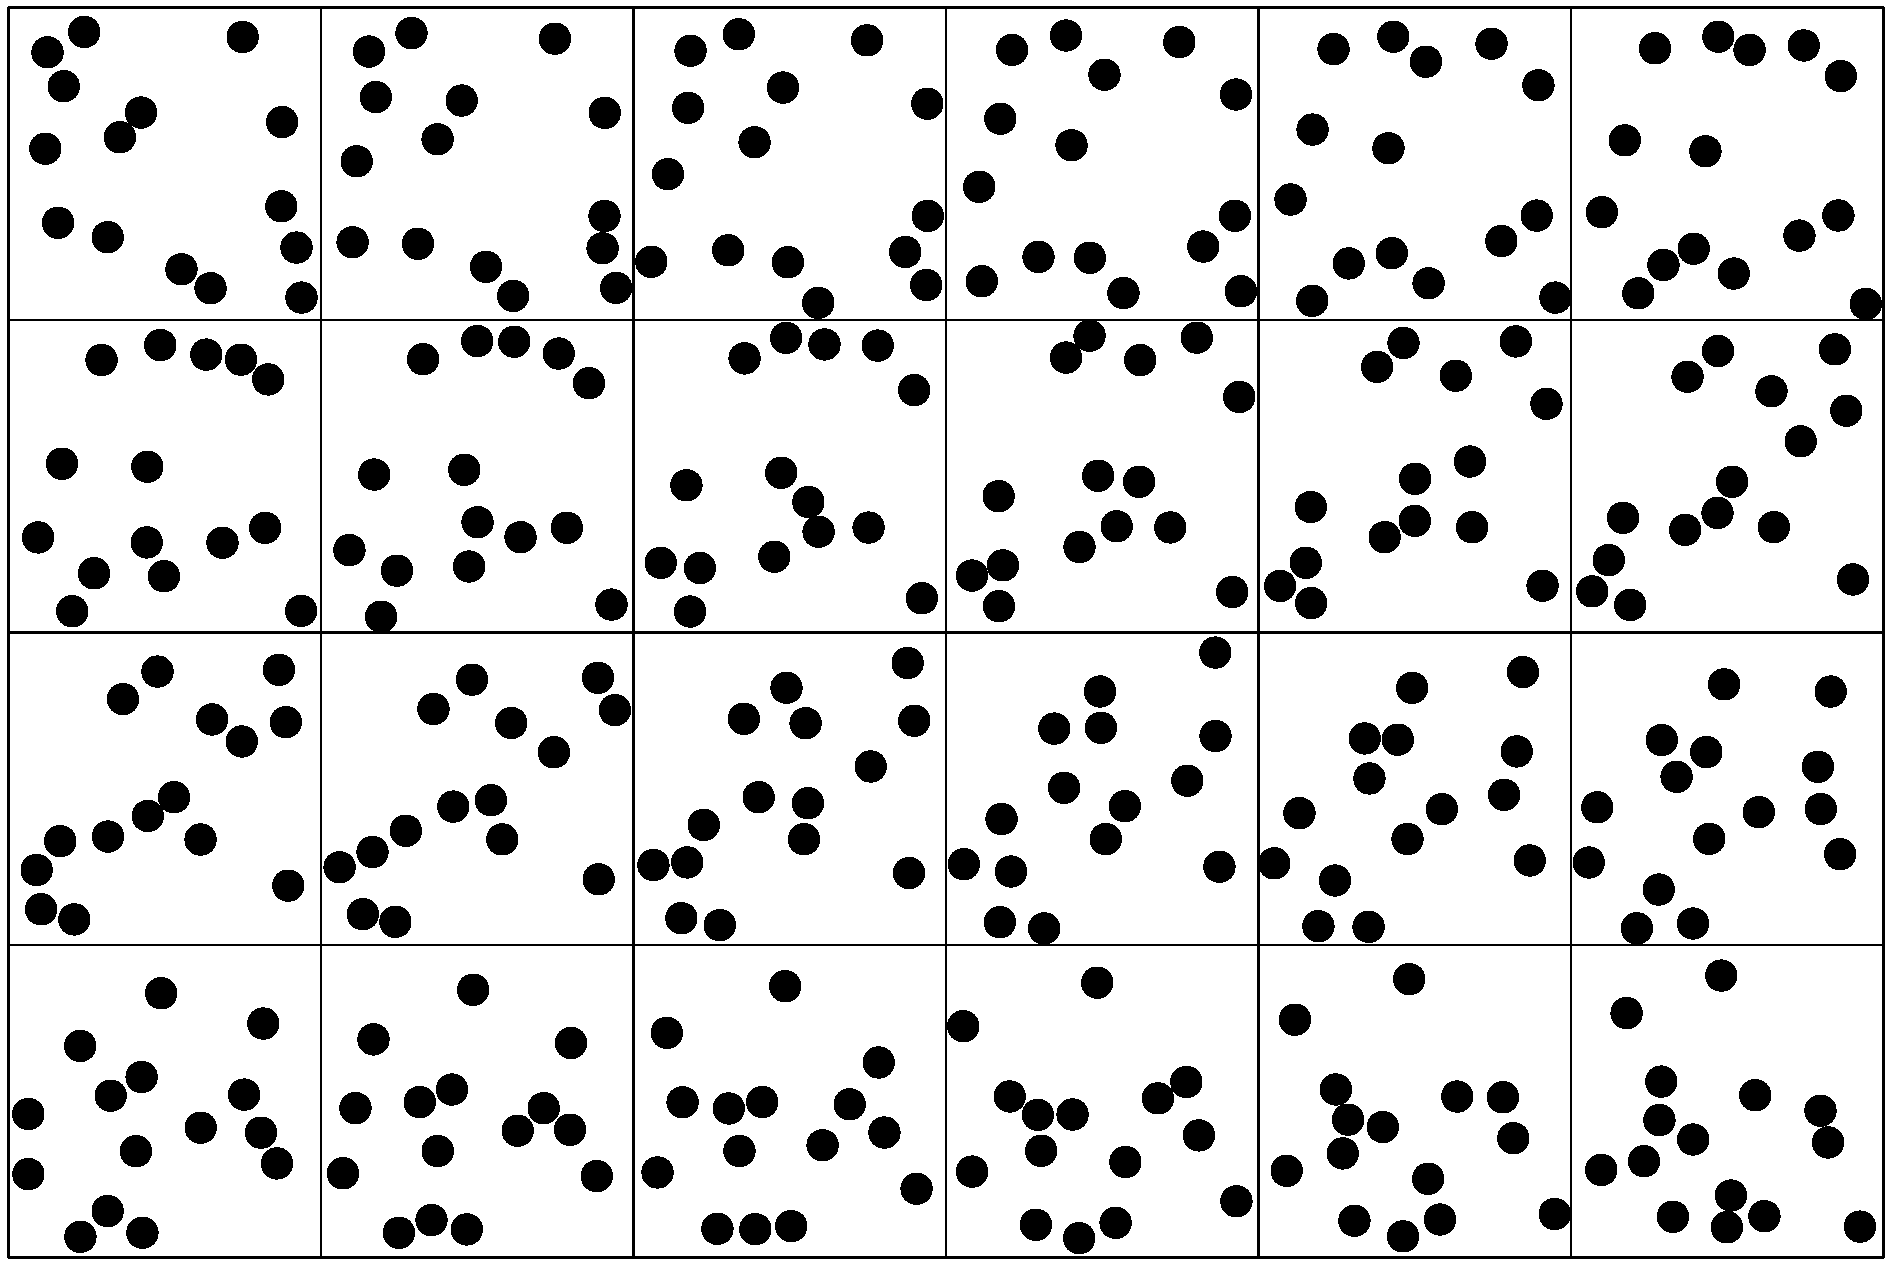
\includegraphics[width=16cm]{brownian}
    \caption{Раскадровка примера визуализации броуновского движения\label{brownianfig}}
\end{figure}

\section{Перспективы и дальнейшее возможное развитие}

\subsection{Расширение возможностей многопользовательского режима}

Сейчас модели, с которыми проиходит взаимодействие в комнатах многопольовательского режима, исчезают вместе с отключением сервера.
Можно реализовать сохранение в моделей в базе данных, что позволит их восстановить при последующем запуске программы.
Из-за иммутабельной природы модели, можно использовать git-подобное хранилище.
Вместо хранения модели целиком, можно хранить в базе данных множество разниц, которые указывают на предыдущею разницу.
Т.е. для восстановления конкретной модели требуется знать идентификатор последней разницы, которая восстановиться из цепочки разниц.
А для сохранения изменённой модели из сохранённой достаточно записать новую разницу в базу данных,
назначив идентификатор предыдущей, как идентификатор разницы из которой была восстановлена модель.

Кроме этого, можно добавить чат, автоматизировать экспорт и импорт модели из одиночного режима.

\subsection{Аналог игры <<Чапаев>>}

Реализованную демонстрацию возможностей движка можно расширить онлайн-игрой.
Одно из самых простых и очевидных, это пошаговая игра, в которой надо выбивать фигуры противника с игрового поля~--
в реальном мире такая называется <<Чапаев>>~\cite{wiki-chapaev}.
В онлайн-мире реализация подобной игры может быть известна под названием <<Смешарики>>~\cite{smeshariki-fandom}.
Кроме подобных правил, можно реализовать интеграцию с социальными сетями, такими как
VK (используя игровую платформу~\cite{vk-games}) и Telegram (используя Gaming~Platworm~\cite{tg-games}).

\subsection{Оптимизация производительности}\label{optimization}

Из-за ограниченного времени, при реализации алгоритма не было приоритета сделать его оптимальным.
Поэтому многие места реализованы тривиально, что могло привести к лишним вычислениям, что плохо отразилось на производительности.
Например, во многих местах, где требуется перебирать пары,
можно не перебирать пары одинаковых элементов и пары, которые уже были учтены, но с другим порядком элементов.
При использовании символьных вычислений, вывод выражения вычисляется каждый раз заново, несмотря на то, что выражения используются каждый раз одни и те же.
Это можно оптимизировать, сохраняя результат, т.е. использовать мемоизацию.
Далее, для поиска узких мест алгоритма можно использовать профилирование и пытаться оптимизировать их.

Другой подход увеличения производительности~-- использовать не одно процессорное ядро, а несколько, т.е. использовать параллелизм.
Хоть и в пункте~\ref{concurrent12} указано, что OCaml является языком с однопоточной средой выполнения,
готовится релиз OCaml 5.0 (Multicore OCaml), в котором будет поддержана многопоточная среда выполнения~\cite{infoqmulticore}.
А это значит, что многие места реализованного алгоритма можно будет распараллелить.
Например, используя пул доменов (потоков) библиотеки domainslib~\cite{domainslibgithub},
можно вычислять одновременно такие вычисления как обнаружение столкновений, или даже поиск корней уравнения.
В JavaScript среде выполнения параллелизм не поддерживается, поэтому придётся написать абстракцию пула доменов,
которая для клиентской (браузерной) среды выполнения будет использовать 1 поток, а для серверной несколько потоков.

\subsection{Обобщение}

Потенциал подхода не ограничен системой с одной лишь силой трения.
Благодаря механизму задания правил, движок можно модифицировать так, чтобы тела передвигались по другим формулам.
Можно модифицировать механизм задания правил, чтобы он использовал множество действующих на тело сил.
Модифицируя движок, можно делать модель ближе или дальше к реальности.
Так же, реализованный движок не поддерживает связи между телами, которые
могут образовываться когда после столкновения они движутся вместе, т.е. одно толкает другое.
Кроме этого в движке можно поддержать неупругие столкновения (т.е. ввести для тел, точек, отрезков коэффициент восстановления).
Теоретически можно переписать движок так, чтобы поддерживалось трёхмерное пространство.
Тогда, следует вместо формулы~(\ref{bodybodycollisioncoords}) использовать подобную, только для сферы и т.д.

% \subsection{Формальная верификация частей алгоритма}

% \TODO
